\documentclass{article}

\begin{document}
	\section{Dinero Simulator}
		The Dinero simulator is a cache simulator that lets the use experiment with different cache options such as associativity and block size. We modified various options to determine how it affects the cache miss ratio. The 12 main options given to us to test out are listed below. 
		\begin{itemize}
			\item Split cache with 8Byte blocks directally mapped
			\item Split cache with 8Byte blocks 4 way associative
			\item Split cache with 32Byte blocks directally mapped
			\item Split cache with 32Byte blocks 4 way associative
			\item Split cache with 128Byte blocks directally mapped
			\item Split cache with 128Byte blocks 4 way associative
			\item Unified cache with 8Byte blocks directally mapped
			\item Unified cache with 8Byte blocks 4 way associative
			\item Unified cache with 32Byte blocks directally mapped
			\item Unified cache with 32Byte blocks 4 way associative
			\item Unified cache with 128Byte blocks directally mapped
			\item Unified cache with 128Byte blocks 4 way associative
		\end{itemize}
		The split caches were comprised of 16KB instruction cache and 16KB data cache. The unified caches were 32KB large. These experiments were ran using this command for split cache.
		\begin{lstlisting}[language=bash]
			cat ../../project/trace.din | ./dineroIV -l1-dsize \textbf{<DATA_CACHE_SIZE>} -l1-dbsize \textbf{<DATA_BLOCK_SIZE>} -l1-dassoc \textbf{<DATA_ASSOC>} -l1-isize \textbf{<INS_CACHE_SIZE>} -l1-ibsize \textbf{<INS_BLOCK_SIZE>} -l1-iassoc \textbf{<INS_ASSOC>} -informatd
		\end{lstlisting}
		And this command for unified cache.
		\begin{lstlisting}[language=bash]
			cat ../../project/trace.din |  ./dineroIV -l1-usize 32K -l1-ubsize 128 -l1-uassoc 1 -informatd
		\end{lstlisting}
		\par
		The result of the experiment with the dineroIV simulator was consistant with the theroy tought in class. The results are laied neatly in this graoh below. 
		\being{figure}[H]
			\label{uni-cache-metrics}
			\begin{center}
				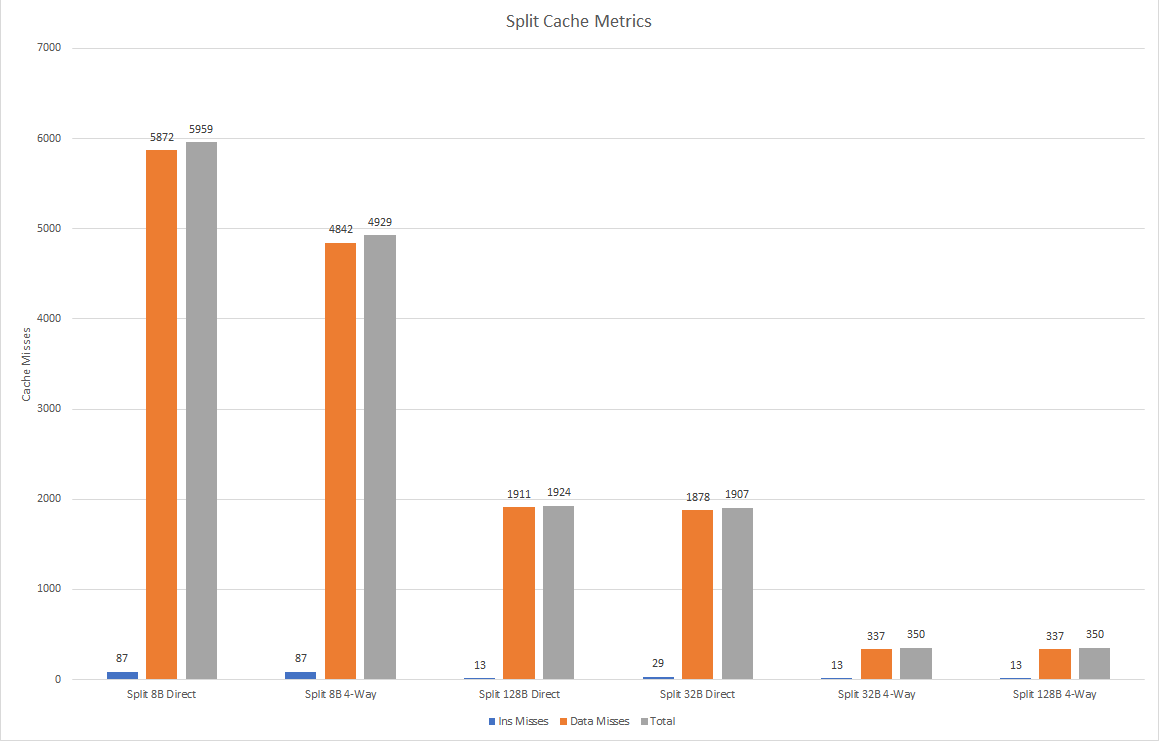
\includegraphics[width=6cm]{uni-cache-metrics.png}
				\caption{Metrics of a unified cache}
			\end{center}
		\end{figure}
		A general trend that can be seen in Figure \ref{uni-cache-metrics} is that as the associativity increases the miss rate drops. This is because when the associativity is increased a cache line is less likely to fight another line for a spot in the cache. This type of cache miss is known as conflict misses because 2 lines are confilicting for a spot in the cache. Another trend that can be seen is that as the size of the cache line is increased, the miss rate drops. This is because as the cache line size is increased the spacial locality of that line is also increased. When data is accessed, it is highly likly that some data next to or around that data will be accessed next or in the near future. By increasing the blick size, we can take advantage of this fact and load possible future memory access into the cache befoire they are actually accessed. This type of cache is usually used in L2 caches because the data and instructions dont need to be seperated.  
		\par
		Contrary to the L2 cache, the L1 cache is usually  
		
\end{document}